\chapter{Variational Greedy InfoMax}

\section{Motivation} %\section{Problem setting}
	In the previous section we discussed two categories of representation learning though deep learning. First, we discussed the autoencoder and its variational counterpart, which minimise the reconstruction error. Secondly, we discussed Contrastive Predictive Coding and Greedy InfoMax, both of which optimise the Info NCE objective. This category seeks to maximise the mutual information between the encodings of data patches that are temporally nearby. The latent representations obtained from all four methods can then be utilised for downstream tasks \cite{bengioRepresentationLearningReview2013, weiRecentAdvancesVariational2021, oordRepresentationLearningContrastive2019, lowePuttingEndEndtoEnd2020}
	
	% repr learn autoenc + vae (disentenglement)
		The autoencoder's sole objective is to define representations to reconstruct the original data. As a result, the representations may serve well for data compression, however, no additional constraints are enforced, such as feature disentanglement and thus the latent space may still be hard to work with for downstream tasks \cite{tschannenRecentAdvancesAutoencoderBased2018}. Meanwhile, VAEs' additional regularisation term, results in representations which break down or disentangle each feature into a narrowly defined variable and encodes them as separate dimensions \cite{weiRecentAdvancesVariational2021}. This additional constrained may result in better suited representations for downstream tasks. % TODO: I could reformulate this, and mention meta priors such as in this paper: https://arxiv.org/pdf/1812.05069.pdf

	% cpc contrasts noise -> smaller architect
		Both autoencoders and VAEs merely learn to reconstruct the data. Hence, all the "information" that is important to reconstruct the data will be maintained in the latent representation, whether the information is useful for the downstream task or not. Meanwhile, optimising latent representations for the InfoNCE objective will maintain shared information between temporally nearby patches, while discarding local noise. Reconstruction is thus not needed for training. This strategy has the tremendous benefit that a decoder block is not required, resulting in a significantly simplified architecture, meanwhile maintaining state-of-the-art performance \cite{stackeEvaluationContrastivePredictive2020}. A second benefit of these mutual information maximisation models is that they are directly compatible with sequential data.
		
	% lead to interpretabil
		Both categories (reconstruction and information maximisation algorithms) possess the ability to obtain useful representations for various downstream tasks. However, the content of these representations may not always be intuitive to humans and their structure may be difficult to comprehend. While CPC and GIM are considered state-of-the-art, their performance comes at a cost of having the least interpretable representations. Autoencoders maintain interpretability by using a decoder to reveal the information contained in the latent representation. The same transparency can also be achieved with VAEs. Additionally, by using a standard Gaussian as a prior and constraining the latent distributions to be similar to this prior, we can interpolate between representations and observe the effects through the decoder. As such, we can observe the specific information that is contained in each of the representation's features. VAEs can also result in disentangled features, further enhancing interpretability \cite{grossuttiDeepLearningInfrared2022}. In contrast, CPC and GIM do not contain a built in decoder mechanism, nor pose constraints on the latent space, significantly reducing interpretability.
		


\section{Towards decoupled training for probabilistic representations}
	% Our contribution
		In what follows next we introduce Variational Greedy InfoMax (V-GIM), maintaining the state-of-the-art performance obtained from optimising InfoNCE, while leveraging the interpretable and disentangled benefits from VAEs. This is achieved by optimising a novel loss function, \textit{Variational-InfoNCE}, a combination of InfoNCE and the regularisation term from VAEs. Additionally, by splitting up the neural network into modules, as introduced in \cite{lowePuttingEndEndtoEnd2020}, we greedily optimise each module with its own instance of this loss function. As a result, the interpretability benefits from VAEs will also be applicable in-between modules. This is in contrast to VAEs where solely the final output representations are interpretable.		
				
	% How:
		% still maximise mutual information between zt, ztk, but predictions no longer fixed datapoints.
		% xt -> cpc model -> q( . | xt) = mui, sigmai
		
		As discussed in the section on Contrastive Predictive Coding (CPC), a patch of sequential data $\xt$ is encoded through $g_{enc}(\xt) = \zt$ and aggregated over previous encodings through auto-regressor $g_{ar}(\z_1  \dots \zt) = \ct$, where both $\zt$ or $\ct$ may serve as representations for downstream tasks. The encoder function $\genc$ is represented as neural network, eg via a CNN, and $\gar$ for instance as a GRU. % todo: are gru and cnn used before?
		Finally, the encoding functions $\genc$ and $\gar$ are obtained by optimising a global loss function, the InfoNCE loss, end-to-end via backpropagation. 

		% split in modules
			Instead, in this study, we split up $\genc$'s network architecture by depth into $M$ modules 
			$$g_{enc}^1(\cdot),~ g_{enc}^2(\cdot),~\dots,~g_{enc}^M(\cdot)$$ 
			and prevent gradients from flowing between modules, as introduced in \cite{lowePuttingEndEndtoEnd2020}. An additional optional $M+1$'th module $\gar$ can be appended to the architecture. Each module is greedily optimised via a novel loss function, $\Lvnce$, which we will define in a following subsection. Each module's output serves as input for the successive module, as presented in the following equations. %#, and depicted in figure \ref{fig:variationalgim}.			
				%			\begin{figure} % fig: overview multiple modules
				%				\centering
				%				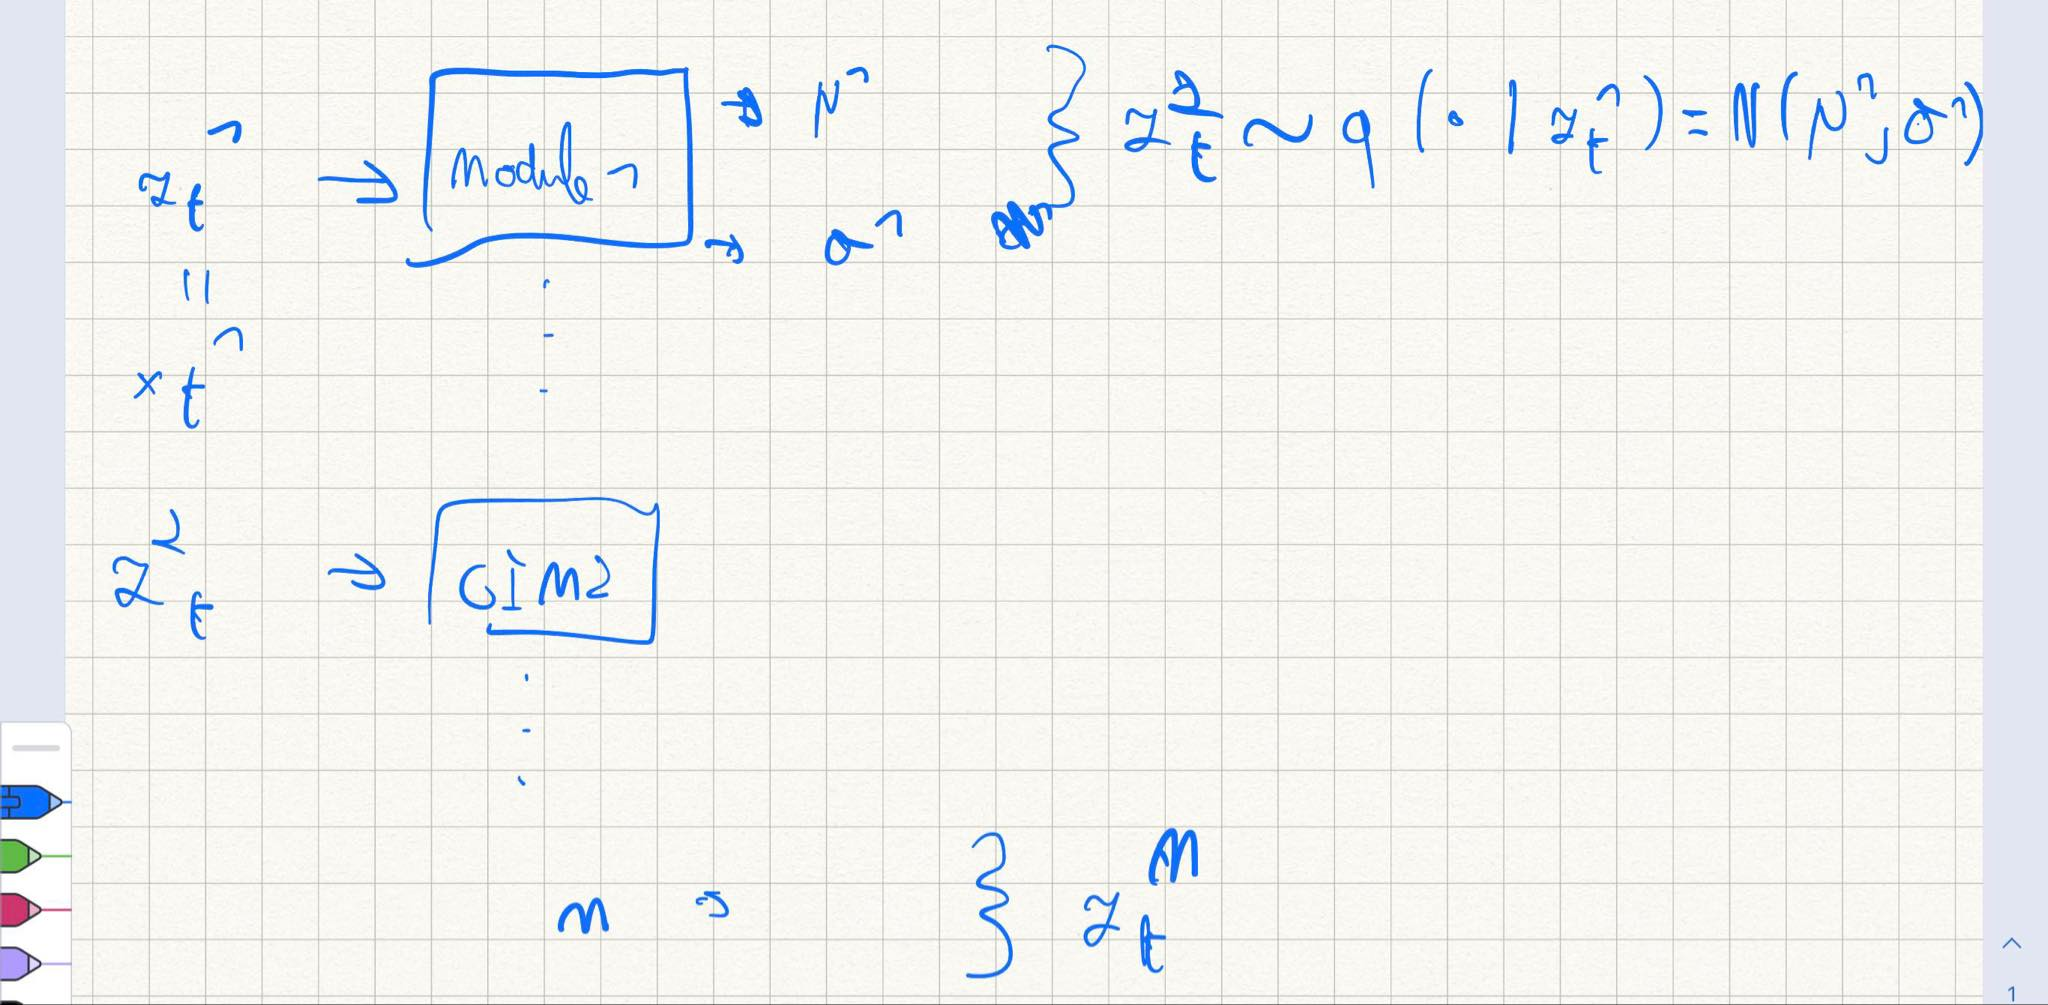
\includegraphics[width=0.7\linewidth]{temp_variational_gim}
				%				\caption{}
				%				\label{fig:variationalgim}
				%			\end{figure}
			\begin{align*} % g_enc1, ...
				g_{enc}^1(\xt) &= \zt^1 \\
				g_{enc}^m(\zt^{m-1}) &= \zt^m \\
				g_{ar}(\z_1^M ~ \dots ~ \zt^M) &= \ct
			\end{align*}
			
			The final representation $\ct$ is obtained by propagating $\xt$ through each modules as follows:
			$$ g_{ar}(g_{enc}^M ( \dots	g_{enc}^2(g_{enc}^1(\xt)))) $$
			
			% TODO: WANNEER OVER GRADIENTS BEGINT, A SINGLE MODULE IS DEFINED AS FOLLOWS.. MET F(z m-1) -> (mu, sigm)
			
			
					
		% Distributions
			Additionally, taking inspriation from VAEs, the outputs from $\gencm$ and $\gar$ are in fact samples from a distribution denoted by $q(\zt^m \mid \zt^{m-1})$, defined as a multivariate Gaussian with diagonal covariance matrix, as follows:
			$$\sampleqdot{\zt^{m-1}} = \normalfatmusigma$$
			with $\mufat$ and $\sigmafat$ dependent on $\zt^{m-1}$, specified in more detail in a following subsection.
			The outputs for $\gencm$ and $\gar$ are obtained by sampling from this distribution, denoted respectively, as follows:
 			\begin{align} % z ~ q AND c ~ q
			 	\sample{\zt^m}~ & \qfromzmneg  \label{eq:sample_z_from_q} \\
			 	\sample{\ct}~ & \qfromzM
			 \end{align}
			Modules are thus stochastic and computing $g_{enc}^m(\zt^{m-1})$ twice will likely result in two different representations of $\zt^m$. This is in contrast to CPC and GIM's encodings which remain fixed depending to the input \cite{oordRepresentationLearningContrastive2019, lowePuttingEndEndtoEnd2020}.
		
		% How distributions: predict q + sample
			We achieve these stochastic modules by defining each module $\gencm$ consisting of two blocks. The first block receives as input $\zt^{m-1}$ and predicts the parameters $\mufat$ and $\sigmafat$. These two parameters describe the distribution $\qfromzmneg$. Since we defined $q$ as Gaussian with a diagonal covariance matrix, the distribution can be fully described by those two vectors. The second block samples 
			$\sample{\zt^m} \sampleqdot{\zt^{m-1}}$ from this distribution and produces an output representation. This is depicted in figure \ref{fig:single_variational_module}.
			
						
\begin{figure}[h]
	\centering
	\tikzstyle{arrow} = [thick,->,>=stealth]
	\begin{tikzpicture}[
		AnnNode/.style={trapezium, draw=black,
			trapezium stretches=true,
			minimum width=2cm, 
			minimum height=1.5cm,
			rotate=-90,
			trapezium angle=75,
			very thick},
		SamplingBlock/.style={rectangle, draw=black,
			minimum height=1cm, minimum width=2cm,
			very thick},
		]
		
		\node[AnnNode] (enc) {\rotatebox{90}{ANN}};
		\node[SamplingBlock] [right of=enc, xshift=2.5cm] (sample) {$\zt^m \sim \sampleqdot{\zt^{m-1}}$};
		
		% enc edges
		\draw[->] ++(-2.5, 0) -- (enc.south) node[above, midway] {$\zt^{m-1}$};
		\draw[->] 
		[transform canvas={yshift=.7em}] 
		(enc.north) -- (sample.west) node[above, midway] {$\mufat$};
		
		\draw[->] 
		[transform canvas={yshift=-.7em}] 
		(enc.north) --  (sample.west) node[below, midway] {$\sigmafat$};
		
		\draw[->] 
		(sample.east) --  ++(1.5, 0) node[above, midway] {$\zt^m$};
		
		
		
		
	\end{tikzpicture}
	\caption{A single module.}
	\label{fig:single_variational_module}
\end{figure}

			
		% define ztm~q() = gaussian., --> z = mu + sigma*noise
			In practice, sampling from $q$ is achieved through a reparametrisation trick, as introduced in \cite{kingmaAutoEncodingVariationalBayes2022}. The equation to compute $\zt^m$ then becomes:
			\begin{equation*}
				\zt = \mufat + \sigmafat \odot \epilonfat
			\end{equation*}
			where $\epilonfat$ corresponds to a sampled value $\samplestandardnormal{\epilonfat}$ and $\odot$ is element-wise multiplication. The procedure to obtain $\ct$ is analogous to $\zt^m$ which we described above.
			
			
		Because of this probabilistic approach, a single patch of data $\xt$ will have multiple representations $\zt^M$, providing increased variance in the representations. This can potentially benefit downstream tasks, particularly when labelled data in scarce \cite{weiRecentAdvancesVariational2021}, leading to improved performance. % TODO: this benefit should be moved to benefits section.
			

		
		
\section{The learning objective}
	Instead of training the neural network end-to-end with a global loss function, the network is split up into modules, which each are optimised greedily with their own personal loss function. Through the introduction of the novel \textit{Variational-InfoNCE} loss, mutual information between temporally nearby representations is maximised, while regularising the latent space to be approximate to the standard Gaussian $\standardnormal$. The Variational-InfoNCE loss is defined as follows:
	
	\begin{equation} % variational_gim_loss % TODO: die k's is niet echt correct/onvolledig
		% \mathcal{L}(\ztk^{m-1}, \zt^{m-1}) = 
		\Lvnce^m =
		\underbrace{\reconstrgim}_{\text{Maximise } I(\ztk^m, \zt^m)} + \underbrace{\beta ~ \latentspaceconstraintgim}_{\text{Regularisation}}
		\label{eq:variational_gim_loss}
	\end{equation}

	$m \in \naturalset$ refers to the $m$'th module. $k \in \naturalset$ corresponds to the number of patches in the future the similarity score $\fkm$ must rate. $\ztk^m$ and $\zt^m$ are encoded samples produced by $g_{enc}^m(\ztk^{m-1})$ and $g_{enc}^m(\zt^{m-1})$, respectively. $X$ is a set of samples ${ \left\{ \ztk^m, \z_1^m, \z_2^m, \dots \right\} }$ where $\zj^m \neq \ztk^m$ are random samples.


	The similarity score $f_k^m(\cdot)$'s definition is identical to \cite{lowePuttingEndEndtoEnd2020}:
	
	$$ f_k^m(\ztk^m,\zt^m) = \exp({\ztk^m}^TW_k^m\zt^m) $$
	
	$\Lvnce^m$ consists of two terms. The first term ensures that encodings of temporally nearby patches contained maximised mutual information. The second ensures that those encodings are all close to the standard normal $\standardnormal$. Finally, $\beta$ is a hyper-parameter which decides the relative importance between the two terms. $\beta >> 1$ will weight more importance to regularisation, but may result in posterior collapse \cite{lucasUnderstandingPosteriorCollapse2022}. On the other hand $\beta \approx 0$ will attach more importance to the mutual information maximisation term while forgetting about the regularisation term. When $\beta = 0$, V-GIM is identical to GIM but with an altered neural network architecture which supports probabilistic encodings.
	
	\subsection{Gradient \textbf{TODO}}
		The gradient of the first term in $\Lvnce^m$ can be approximated through mini-batches, and optimised directly in PyTorch. With regards to the second term, since $\qfromzmneg$ is a Gaussian, a closed form solution exists \cite{kingmaAutoEncodingVariationalBayes2022}, the term can be differentiated without approximated method.
		
		
		%Where the KL divergence for a single sample $x^{(i)}$ is approximated as follows:
		% https://arxiv.org/pdf/1312.6114.pdf, from example
		\begin{equation}
			\frac{1}{2}\sum_{j=1}^J \left( 1 + \log((\sigma_j^{(i)})^2) - (\mu_j^{(i)})^2 - (\sigma_j^{(i)})^2 \right) 
		\end{equation}
		
		\begin{equation} % REAL BUT MUST REMOVE THE (i)	
			\kl{\normal}{\standardnormal} = \latentspaceconstraintclosedform
		\end{equation}
		
		
		where $z^(i,l) = \sigma ^{(i)} \odot \epsilon^{(l)}$ and $\epsilon^(l) \mathcal{N}(0, I)$
		
		\textbf{todo: variables should maybe be bold.}
		
		
		%	TODO: DUS DIE KL DIVERGENCE CLOSED FORM NOTATIE, MAAR BIJ SAMPLING ZOU OOK DEFINITIE VAN Z = MU + SIGMA*ERR GEVEN
	
	
	\subsection{Continuous space around the origin} \label{cha:contin_space}
		% TODO
		\textbf{@Bart, when you read this, make sure to be very critical, as I am not 100\% convinced of what I wrote in this paragraph.}
		
		
		% around N()
			As we discussed earlier, the encodings $\sample{\zt^m}~ \qfromzmneg$ generated by each module $m$ are samples from a Gaussian distribution (which may not necessarily be the standard normal), and may thus have multiple representations. These samples are optimised to be as close as possible to the standard normal $\standardnormal$. 
	
		% smooth changes
			Consider $\ztk^{m-1}$ and $\zt^{m-1}$ which each serve as input for a fully trained module $\gencm$. These two inputs are temporally nearby, and thus, due to the slowly varying features assumption \cite{zhangSlowFeatureAnalysis2012} have a lot of information in common. This means that the correspondence score of their encodings, estimated by the scoring function $\fkmblank$, should also be high. However, as depicted in \ref{fig:gaussian-neighbourhood}, the encodings for $\ztk^{m-1}$ correspond an entire space $ \{ {\ztk^m}^{'},~{\ztk^m}^{''},~\dots \}$ centred around a particular mean vector $\mufat$. If $\Lvnce^m$ is optimal, this means that given encoding $\zt^m$, $f_k^m({\ztk^m}^{'}, {\zt^m})$ should be  large, but also $f_k^m({\ztk^m}^{''}, {\zt^m})$, while remaining small for random encodings $\zi^m \neq \ztk^m$. The correspondence scores must thus be similar for all encodings in a particular neighbourhood, meaning they all have similar mutual information to $\zt^{m}$. This is important, because it will ensure smooth transitions in the latent space. Furthermore, optimising this loss function also maximises the mutual information between outputs of successive modules $I(\zt^{m-1}, \zt^{m})$ \cite{lowePuttingEndEndtoEnd2020}, and the smooth transitions will reflect on the original representations $\xt$.			 
		
		\begin{figure} % gauss neighbourhood
			\centering
			\includegraphics[width=0.7\linewidth]{"gaussian neighbourhood"}
			\caption{}
			\label{fig:gaussian-neighbourhood}
		\end{figure}
		
		% gaps
			Finally, since the set of encodings $ \{ {\zt^1}^{'},~{\zt^1}^{''},~\dots \}$ from a single patch $\xt$ corresponds to a large neighbourhood in the latent space, and since the latent space is fairly small (standard normal) representation distributions from different data points are likely to be pushed around, trying to utilise the limited space as best as they can. This results in a less likely chance of obtaining holes in the latent space.
			
			The end result is a continuous space around the origin, which is a crucial observation. It will serve as the main argument for why V-GIM's representations are interpretable, while traditional techniques such as CPC and GIM do not have these guarantees. 

			


		
	
	
	
\section{Computational benefits}
	Each module in V-GIM is greedily trained through the variational InfoNCE loss. his allows for decoupled, memory-efficient asynchronous distributed training and mitigates the vanishing gradient problem, which are benefits introduced by GIM \cite{lowePuttingEndEndtoEnd2020}. However, V-GIM adds a constraint to the embedded space produced by each module, leading to additional practical benefits. Since V-GIM adopts a greedy training approach, these benefits apply not only to the final module's output but also to the outputs of intermediate modules.
	

	\subsubsection{Interpretability of final and intermediate encodings}
		By carefully optimising the embedded space with the properties discussed in section \ref{cha:contin_space}, V-GIM creates a space where sampling from a point around the origin is likely to correspond to a data point that is similar to the dataset. A decoder trained on this space will generalize well to unseen data when given an encoding it has never seen before. This is in contrast to GIM and CPC, which do not impose constraints on the encoding space. While a decoder can also be trained on the encodings produced by GIM or CPC, the embedded space is highly unpredictable, and sampling a random encoding around the origin is not guaranteed to result in a meaningful decoding. This makes it challenging to interpret the underlying structure of the encodings. Figure \ref{fig:no-regularisation} illustrates this difference between V-GIM and GIM/CPC.
		
		% Without regularisation, the shape of the embedded space is unpredictable, and thus we do not known what from which data points samples are taken when choosing a random encoding, or when interpolating between two well formed encodings representations (aka, two encodings obtained by encoding data points from the dataset).
	
		\begin{figure} % regul vs no regul
			\centering
			\includegraphics[width=0.7\linewidth]{"no regularisation"}
			\caption{Left is without regularisation (eg space obtained from a single module from GIM). Right is with regularisation (eg: V-GIM). A decoder's objective is to learn a reversed mapping function from the blue z-space to the green x-space. The decoder is only trained on the blue cloud and not data points around it so it may not generalise well to those representations. }
			\label{fig:no-regularisation}
		\end{figure}
	
		The interpretability of V-GIM's encodings has significant implications, as we can not only assess the information contained in an encoding through a decoder but also attempt to understand the underlying structure of the encodings. Similar to how this is done in VAEs, we can alter one component of a random encoding at a time and observe the effect through the decoder, allowing us to understand the underlying structure of the encodings.
		
		Furthermore, since V-GIM's neural network architecture consists of a variable number of modules, each generating interpretable encodings, these benefits are applicable to the encodings produced by intermediate modules, allowing us to observe the internal mechanism of the neural network. Additionally, due to the convolutional neural network (CNN) working, different modules encode different sequence lengths, encouraging different abstractions to be learned at different levels. By having intermediate modules be interpretable, we can analyse these abstractions as well. This is in contrast to VAEs, where only the output encoding is interpretable, and intermediate representations in the architecture are not.

						
	\subsubsection{Disentanglement}
		In section \ref{cha:disentang} on $\beta$-VAEs and disentanglement, Higgins et al. argue that setting the prior $p(\vect{z})$ to an isotropic Gaussian encourages disentanglement in the encodings \cite{higginsBetaVAELearningBasic2022}. When encodings are fully disentangled, this results in each unit component from the encoding to capture a different feature from the original data. This theorem is also applicable to V-GIM and choosing a large value for $\beta$ in $\Lvnce$ applies more pressure for encodings to be disentangled further increasing interpretability.
		
	
	\subsubsection{Improved generalisation through representation variance}
		V-GIM's encodings are samples from a distribution, which means that a single patch of data $\xt$ may have multiple encoded representations $\zt^M$. For downstream tasks with very little labelled data, the variability in representations could serve as an internal data augmentation method, increasing generalisability guarantees of the downstream task.

	
	\subsubsection{Internal batch normalisation mechanism}
		Normalising of inputs is known to accelerate training of neural network by preventing covariate shift from occurring \cite{ioffeBatchNormalizationAccelerating2015, bjorckUnderstandingBatchNormalization2018, lecunEfficientBackProp1998}. However, covariate shift may also occur in the activations of subnetworks, negatively affecting the inputs of subsequent layers \cite{bjorckUnderstandingBatchNormalization2018}. This issue is typically resolved via batch normalisation \cite{santurkarHowDoesBatch2018, bjorckUnderstandingBatchNormalization2018}, a mechanism that also normalises activations of internal layers and allows for higher learning rate during training.
		
		Normalisation is especially important in a greedy setting such as GIM and V-GIM, where modules are independently trained in parallel. Without intermediate normalisation, subsequent modules may learn slower than previous modules, resulting in the subsequent modules not being able to catch up in time to the changes from previous modules made during training. The result would be that modules may have to be trained with different learning rates, resulting in an additional hyperparameter that must be obtained for each module.
		% TODO: ^^ maybe in the paragraph is not clear that parallel training means outputs from module1 are given to module2, while both are training, so module 2 learns from inputs that may change later in the future.
		
		In contrast, V-GIM already contains an internal normalisation mechanism in-between modules. This is indirectly caused by regularising each module's embedded space to the standard normal. This results in encodings with mean of zero and standard deviation of one, that are produced by every module. Finally, the normalised encodings can also be beneficial for downstream tasks. If normalisation is desired, computing the mean and standard deviation over a potentially very large dataset is not required, as this is already built in to the encodings.

	
	

	

		% Copy from Higgins: where the KKT multiplier β is the regularisation coefficient that constrains the capacity of the latent information channel z and puts implicit independence pressure on the learnt posterior due to the isotropic nature of the Gaussian prior p(z)





	%	Better generalisation for downstream tasks
%		- Overfitting: reduction of required labelled data needed. Similar data is similar region, the kl divergence makes regions bigger.
%
%		% copied from a bit higher
%		% Because of this probabilistic approach, a single patch of data $\xt$ will have multiple representations $\zt^M$, providing increased variance in the representations. This can potentially benefit downstream tasks, particularly when labelled data in scarce \cite{weiRecentAdvancesVariational2021}, leading to improved performance. % TODO: this benefit should be moved to benefits section.
%
%		Overfitting during inference:
%		- The same datapoint has multiple (similar) representations, such that learning techniques for downstream tasks will not be able to "memorise" the latent space as easily.
%		
%		- Holes: more predictable inference, such that unseen data is more likely to be near clusters. And thus downstream tasks receive latents that are more similar to what is seen before.
%		= better generalisation






%\textbf{Other sources:} \\
%!!! Abstract on VAE: The fundamental idea in VAEs is to learn the
%distribution of data in such a way that new meaningful data with more intra-class variations can be generated
%from the encoded distribution.
%The ability of VAEs to synthesize new data with more representation variance
%at state-of-art levels provides hope that the chronic scarcity of labeled data in the biomedical field can be
%resolved.
%--> and thus for downstream tasks, has a way of obtaining more labelled data? --> better generalisation


%The goal of representation learning is to be useful for downstream tasks. The most important meta-prior is called ‘disentanglement’ which is an unsupervised learning technique that breaks down, or disentangles, each feature into narrowly defined variables and encodes them as separate dimensions 

%Intuitively, a factorial code disentangles the individual elements that were originally mixed in the sample, just as
%humans recognize complex things by disentangling independent elements. If the dimensions of the latent vector are
%independent of each other, it is factorial disentangled, i.e., a
%good representation. VAEs have made such nonlinear latent
%variable models tractable for modeling complex distributions,
%and efficient extraction of relevant biological information
%from learned features for biological data sets, referred to as
%unsupervised representation learning
%https://ieeexplore.ieee.org/stamp/stamp.jsp?tp=&arnumber=9311619








%We show that the Beta-VAE outperforms principal component analysis (PCA) and learns interpretable and independent representations of the generative factors of variance in the spectra %https://pubs.acs.org/doi/pdf/10.1021/acs.jpclett.2c01328
%


